\documentclass[11pt]{article}
\usepackage{amssymb, amsmath}
\usepackage{graphicx}

\begin{document}
\textbf{{\huge Nguyen Huu Thanh}}


\textit{\textbf{Assignment 3 - Kernel Density Estimator }}
\vspace{5mm}

\section{Show the estimator of $P(x,y)$ by using KERNEL DENSITY ESTIMATOR}
\begin{equation*} 
\begin{split}
P(x, y)& =\frac{1}{n} \sum_{i=1}^{n} K_{h_x}(x-x_i) K_{h_y}(y-y_i)
\end{split}
\end{equation*}


For Gaussian kernel:
\begin{equation*}
\begin{split}
K_{h_x}(x-x_i) &= \frac{1}{\sqrt{2h_x^2\pi}}e^{-\frac{(x-x_i)^2}{2h_x^2}}
\end{split}
\end{equation*}

\begin{equation*}
\begin{split}
K_{h_y}(y-y_i) &= \frac{1}{\sqrt{2h_y^2\pi}}e^{-\frac{(y-y_i)^2}{2h_y^2}}
\end{split}
\end{equation*}

\section{Calculate $E(y|x)$}
\begin{equation*}
\begin{split}
E(y|x) &= \frac{\int_{-\infty}^{\infty}yP(x,y)dy}{\int_{-\infty}^{\infty}P(x,y)dy}
\end{split}
\end{equation*}


For the numerator:
\begin{equation*}
\begin{split}
\int_{-\infty}^{\infty}yP(x,y)dy &= 
\int_{-\infty}^{\infty}y \frac{1}{n} \sum_{i=1}^{n} K_{h_x}(x-x_i) K_{h_y}(y-y_i)dy \\
&= \frac{1}{n} \sum_{i=1}^{n} [K_{h_x}(x-x_i) \int_{-\infty}^{\infty}y K_{h_y}(y-y_i)dy]
\end{split}
\end{equation*}



From Gaussian distribution properties, we have:
\begin{equation*}
\begin{split}
\int_{-\infty}^{\infty}yK_{h_y}(y-y_i)dy &= \int_{-\infty}^{\infty}y\frac{1}{\sqrt{2h_y^2\pi}}e^{-\frac{(y-y_i)^2}{2h_y^2}}dy \\
&= y_i 
\end{split}
\end{equation*}



Hence we can write that 
\begin{equation*}
\begin{split}
\int_{-\infty}^{\infty}yP(x,y)dy &= \frac{1}{n} \sum_{i=1}^{n} K_{h_x}(x-x_i) y_i
\end{split}
\end{equation*}




For the denominator:
\begin{equation*}
\begin{split}
\int_{-\infty}^{\infty}P(x,y)dy &= \frac{1}{n} \sum_{i=1}^{n} K_{h_x}(x-x_i) \int_{-\infty}^{\infty}K_{h_y}(y-y_i)dy \\
&= \frac{1}{n} \sum_{i=1}^{n} K_{h_x}(x-x_i)
\end{split}
\end{equation*}


Therefore:
\begin{equation*}
\begin{split}
E(y|x) &= \frac{\sum_{i=1}^{n}K_{h_x}(x-x_i) y_i}{\sum_{i=1}^{n}K_{h_x}(x-x_i)}
\end{split}
\end{equation*}





\section{Implement estimator of $E(y|x)$}
I have implemented estimator of $E(y|x)$ by using various numbers of $h_x$: $h_x = S_x \frac{k}{M}$ where $S_x$ is standard deviation of X values in \textit{learning\_data2.txt}, $M = 1000$ and value of $k$ run from 1 to $M$. \\
The run time of program is 3 seconds. \\
Best result for Root Mean Squared Error by Leave-one-out cross validation is \textbf{0.02417} when $h_x = S_x * 0.036$ ($S_x$ is is standard deviation of X values).\\
The following image shows the estimating values of Y given X.

\begin{figure}[!ht]
	\centering
	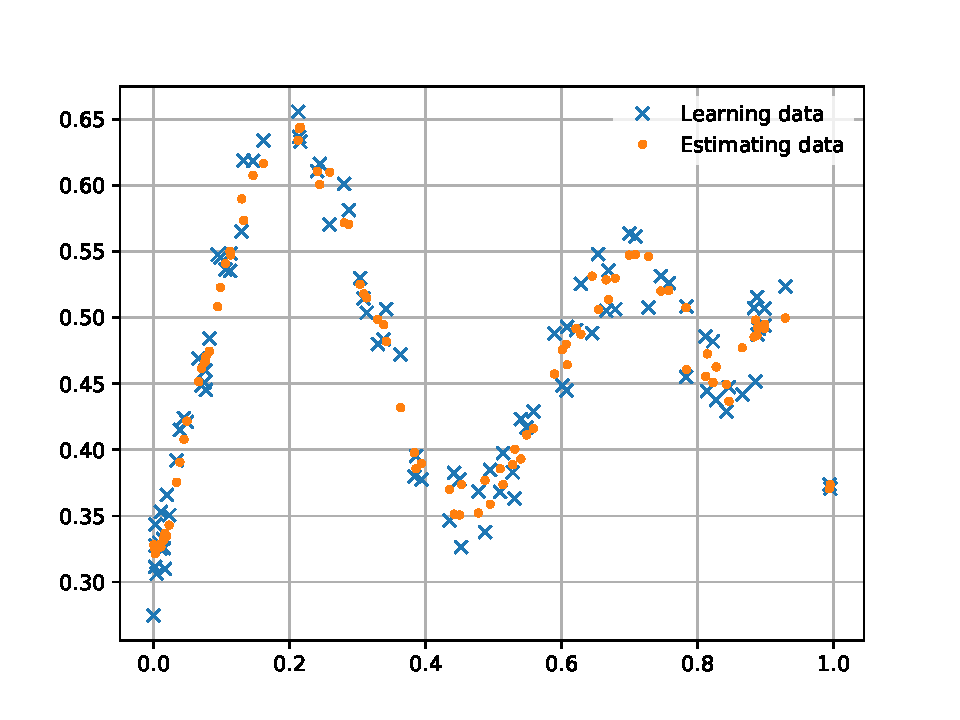
\includegraphics[scale=1.0]{figure.pdf}	
	\caption[29]{Compare leaning data and estimating data, \textbf{RMS = 0.02417}}
\end{figure}


\end{document}